\documentclass[12pt]{article}
\usepackage{graphicx}
\usepackage{array}
\usepackage{makecell}
\PassOptionsToPackage{hyphens}{url}
\usepackage{hyperref}
\usepackage{fancyhdr}
\usepackage{subcaption}
\usepackage{float}
\usepackage{geometry}

\geometry{
 a4paper,
 total={170mm,257mm},
 left=20mm,
 right=20mm,
 top=20mm,
 }

\renewcommand\theadalign{bc}
\renewcommand\theadfont{\bfseries}
\renewcommand\theadgape{\Gape[4pt]}
\renewcommand\cellgape{\Gape[4pt]}
\graphicspath{{pics/}}





\begin{document}


\section*{Development of a smart sensor node for vehicle counting using a CW radar.}
 
\textbf{Description:}
Intelligent Transport Systems (ITS) aim at improving the mobility of people and goods, increasing safety, and reducing the environmental footprint of transport networks(air, water and land) through the use of information and communication technologies. Traffic management is a long pursued objective of ITS for road transport networks. Information regarding the flow of vehicles is essential to any effective traffic management system. To this end, multiple technologies (inductive loops, digital image processing, Lidars, RADARs) have been tried. Vehicle counting through the use of RADARs is the least intrusive method able to operate effectively day and night, under all weather conditions for prolonged periods of time. This project focuses on the design and development of a smart sensor node performing vehicle counting by the use of a radar module operating at 24 GHz, capable of supporting unmodulated CW, FSK and FMCW modes of operation and the experimental evaluation of its effectiveness. Within the context of this diploma thesis the candidate should pursue the following objectives:

\begin{itemize}

\item Brief literature review of the various technologies used for vehicle counting.

\item Literature review of continuous-wave radars working principle, advantages, drawbacks, and applications.

\item Design of a signal processing pipeline that extracts the speed information (magnitude and sign) from the IF outputs of a CW radar.

\item Design of an algorithm that detects passing vehicles using the extracted speed information.

\item Development of an embedded system that implements the previously designed.

\item Experimental evaluation of the system's performance.

 
\end{itemize}


\begin{thebibliography}{999}

\bibitem[Lim \em{et~al.}(2021)]{fmcw}
H. -S. Lim, H. -M. Park, J. -E. Lee, Y. -H. Kim and S. Lee
\newblock Lane-by-Lane Traffic Monitoring Using 24.1 GHz FMCW Radar System.
\newblock {\em IEEE Access} {\bf 2021}, {\em 9},~14677--14687, 10.1109/ACCESS.2021.3052876. 

\bibitem[Fang \em{et~al.}(2007)]{cw}
\newblock A Low-cost Vehicle Detection and Classification System based on Unmodulated Continuous-wave Radar.
\newblock {\em IEEE Intelligent Transportation Systems Conference} {\bf 2007}, {\em 9},~715--720, doi: 10.1109/ITSC.2007.4357739.

\bibitem[Richards \em{et~al.}(2010)]{radar}
Richards, Mark A.; Scheer, James A.; Holm, William A.
\newblock {\em Principles of Modern Radar, Volume I - Basic Principles}; SciTech Publishing: {\bf 2010}.

\end{thebibliography}

\textbf{Requirements:} Embedded System Programming, C programming language, Basic Digital Signal Processing, Understanding of telecommunication electronics primitives(mixers, VCOs, couplers, etc)


\section*{Available Equipment.}

The radar sensor to be used is the K-MC1 radar Front End Module (FEM) from RFbeam. It uses a bistatic configuration with two 30 patch antennas. This module includes an RF low noise amplifier and two $47$ dB IF preamplifiers for both I and Q channels. The unique "RSW" Rapid Sleep Wakeup function with < 4us wakeup time makes this module ideal for battery-operated equipment. The typical duty cycle in RWS mode may be < 1\% with full movement detection capability by sampling the IF signals.

\begin{figure}[H]
\centering
\captionsetup{justification=centering}
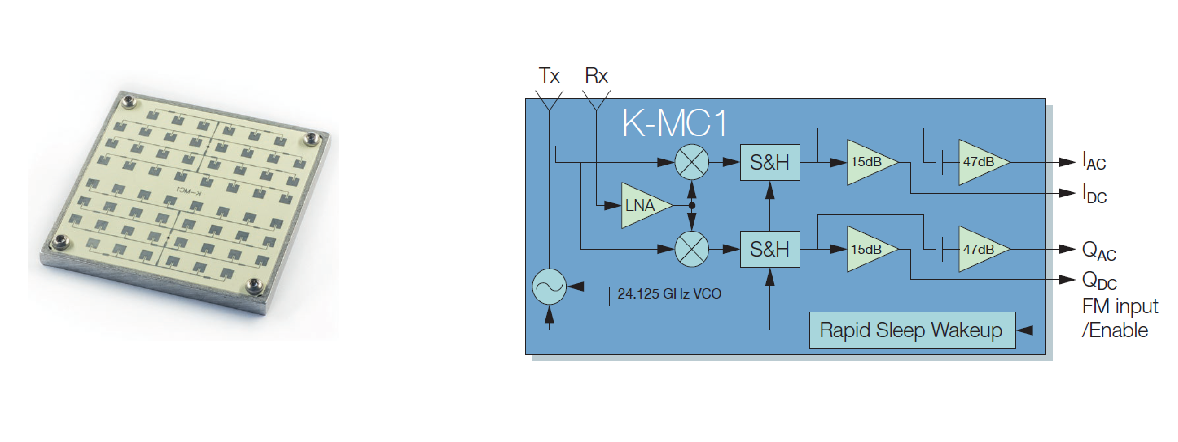
\includegraphics[width=0.9\linewidth,keepaspectratio]{pics/radar_fem.png}
\caption{ K-MC1 radar front end module and its block diagram. \label{image:radar_fem}}
\end{figure}

Furthermore, there is the possibility to choose from various development boards for STM32 micro-controllers, and access is granted to the necessary instruments for the development and debugging of the system (oscilloscope, function generator, etc.).

\begin{figure}[H]
\centering
\captionsetup{justification=centering}
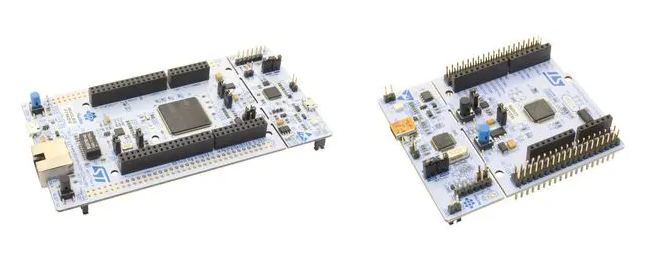
\includegraphics[width=0.7\linewidth,keepaspectratio]{pics/stm32.png}
\caption{ STM32 Nucleo development boards. \label{image:dev_kits}}
\end{figure}

\section*{Development plan.}

Important milestones outlining the development processes are listed here:

\begin{itemize}

\item Literature review.

\item Formulation of the initial system architecture and vehicle counting algorithm.

\item Familiarization with ST's IDE and MCUs.

\item ADC peripheral usage \& sample application that sends the output to the PC.

\item FFT algorithm in C operating on the IF outputs of the radar FEM.

\item Design and implementation of an algorithm that detects passing vehicles using the extracted speed information.

\item Complete system development.

\item Experimental evaluation of the system's performance.

\item Writing of the thesis manuscript.

 
\end{itemize}

\section*{Example application to get started.}

The source code of a sample application will be made available. It is comprised of two parts:

\begin{itemize}

\item C code running in the MCU which, using the ADC, samples the IF outputs of the radar FEM and transmits the sampled data to the PC through UART.

\item A python script that listens to the UART port for data, processes and plots them. 

 
\end{itemize}

\noindent This code is provided to be used for familiarization with the real output of the sensor, serve as a high-level example of the processing pipeline that needs to be implemented in the MCU and capture intermediate and final results from the MCU to visualize the output of the algorithms and signal processing implemented.


\begin{figure}[H]
\centering
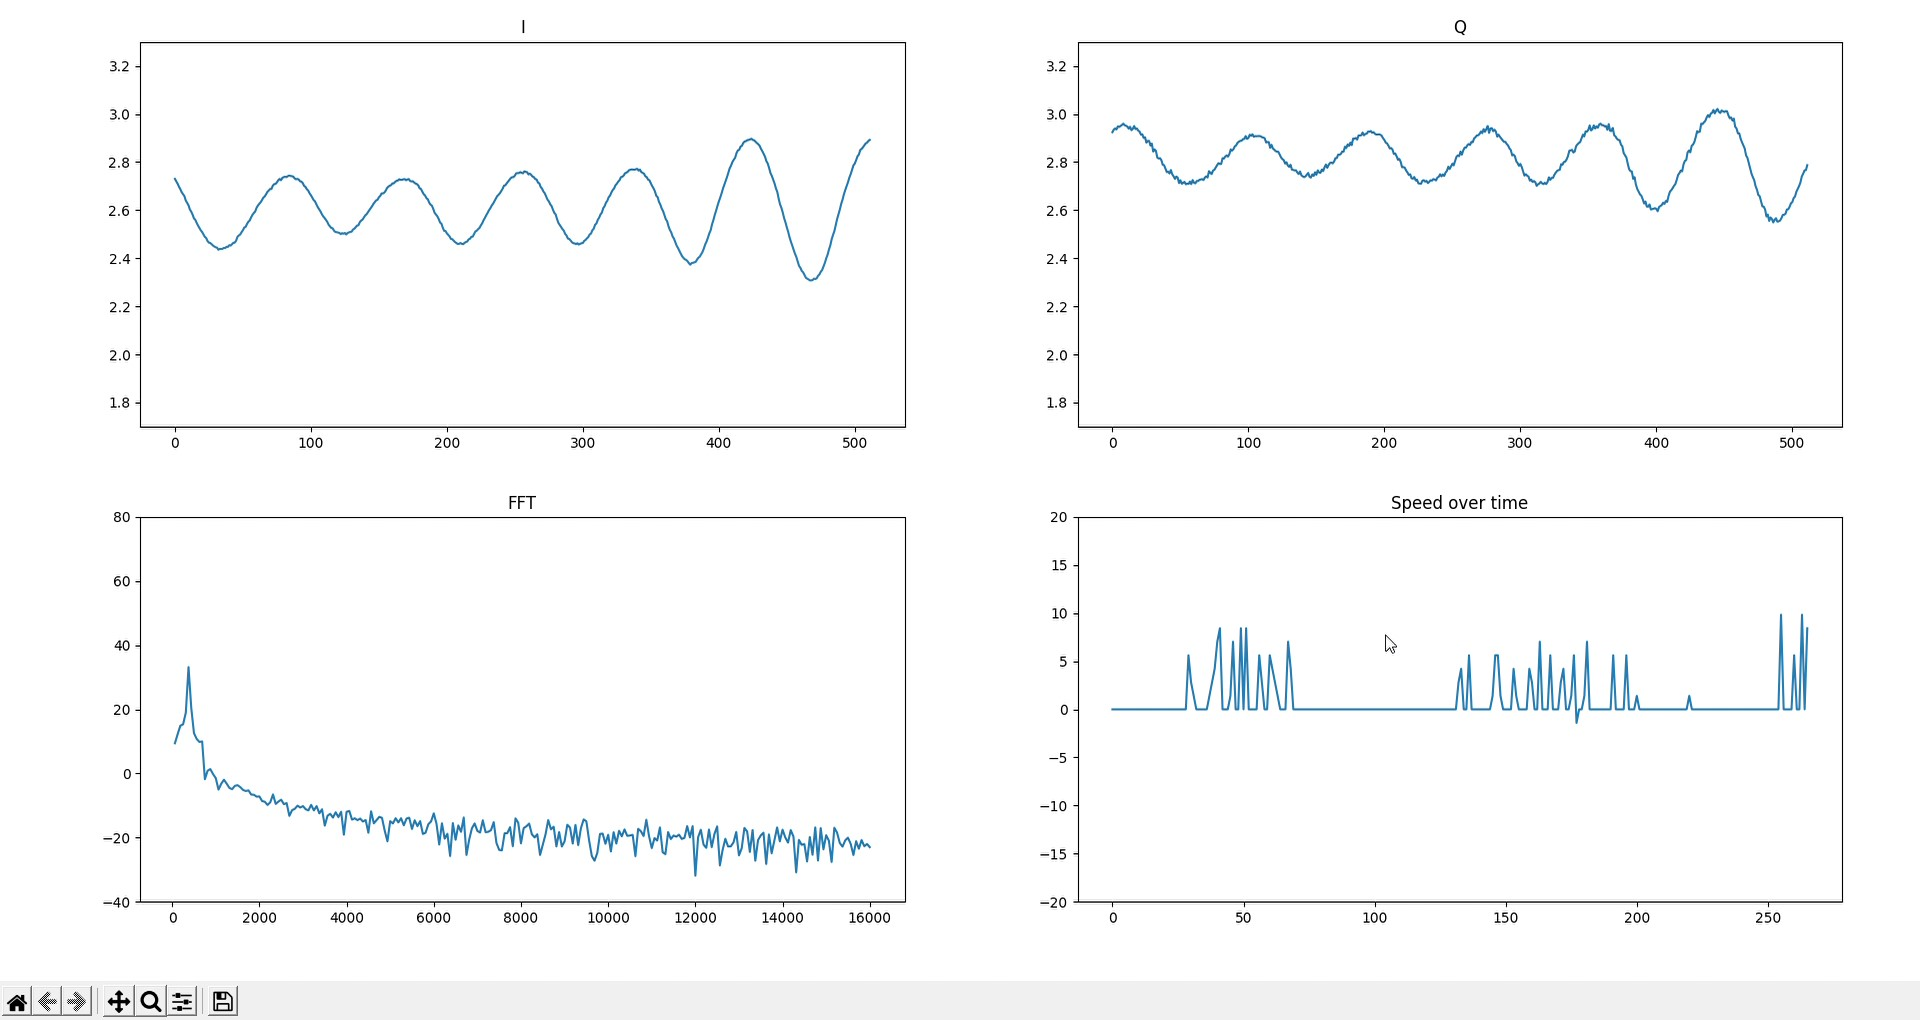
\includegraphics[width=0.9\linewidth,keepaspectratio]{pics/sample_application_output.jpg}
\caption{ Screenshot of the output of the sample application. I and Q IF outputs of the FEM can be seen on the top two images. The bottom left image depicts the FFT of the I IF output and the bottom right image is a graph of the speed of the most reflective object in the radar's beam.  \label{image:smaple_app_out}}
\end{figure}
 
\clearpage
\setcounter{section}{1}

\section*{Proposed table of contents.}
 
\subsection{Introduction}

\begin{itemize}

\item Write about vehicle traffic monitoring, what it is, why it is important, how it can improve our lives.

\item What methods of counting cars are there (inductive loops, cameras, lidars, radars, etc), how do they compare to radars.

\item Problem statement, e.g. Design and develop a system that counts passing cars and measures their speed using a doppler radar.

\end{itemize}


\subsection{Background}

\subsubsection{Doppler radar}

\begin{itemize}

\item Theory regarding Doppler effect.

\item CW radar block diagram and principle of operation.

\item Radar equation.

\end{itemize}

\subsubsection{FFT}

\begin{itemize}

\item Discrete Fourier transform theory.

\item FFT algorithm theory.

\item Spectral leakage and window functions.

\end{itemize}

\subsection{Architecture of the system}

\subsubsection{System overview}

\begin{itemize}

\item Radar FEM and MCU (hardware block diagram), photos.

\item Software block diagram and explanation (from I/Q to speed).

\end{itemize}

\subsubsection{Vehicle counting algorithm from CW radar output}

\begin{itemize}

\item Describe how the detected speed time series is used to detect passing vehicles.

\item Pseudocode/example input output/explanation with pictures.

\end{itemize}

\subsection{Results}

\begin{itemize}

\item Description of the experiment (car/motorcycle passing by).

\item Pictures of the various outputs of the system's sub-blocks with explanation (I/Q with oscillation, fft with peak, speed time series).

\item Power consumption, adequacy to be used as a self-powered device (solar panel).

\end{itemize}

\subsection{Conclusions}

\begin{itemize}

\item State what has been achieved.

\item What are the limitations of the current system.

\item Describe improvements that can be made in the future (FMCW, MIMO, etc).

\end{itemize}


\end{document}
